\documentclass{article}
\usepackage[utf8]{inputenc}
\usepackage{amsmath}
\usepackage{amssymb}
\usepackage{graphicx}
\usepackage{algorithm}
\usepackage[noend]{algpseudocode}
\usepackage[hidelinks]{hyperref}

\title{Problème de clique maximum}

\author{Drissi Mohamed Reda}

\begin{document}

\maketitle
\newpage
\tableofcontents
\newpage
\section{Introduction}
Nous prenons un graphe $G=\{V,E\}$ tel que $V$ est l'ensemble des sommets
et $E$ l'ensemble des arrêtes(Nous ignorons les arrêtes liant une arrête à elle même). \\
Nous nommons les sommets du graphe 1,2, ... n. Cet algorithme permet de trouver une clique
de taille d'au moins $k$. À chaque étape, si nous trouvons une clique de taille d'au moins
$k$, nous arrêtons.
\section{Algorithme et Test}
\subsection{Algorithme}
\begin{algorithm}
\begin{algorithmic}
  \Function{Expand\_clique}{Graph Q}
  \While{$\exists$ v joignable à Q}
    \State trouver $v_{max}$ tel que Le nombre de sommets joignable à la clique $Q \cup \{v_{max}\}$ est maximal
    \State $Q \gets Q\cup \{v_{max}\}$
  \EndWhile
    \State \Return $Q$
  \EndFunction
\end{algorithmic}
\end{algorithm}
\begin{algorithm}
\begin{algorithmic}
  \Function{Alter\_Clique}{Graph Q}
  \State Trouver $v \notin Q$ tel que $\exists! w \in Q$ non adjacent à $v$.
    \If{$v = \varnothing$}
      \State \Return $Q$
    \Else
      \State $Q\gets Q \setminus \{w\}$
      \State $Q \gets Q \cup \{v\}$
      \State $Q \gets$ \Call{Expand\_clique}{Q}
      \State \Return $Q$
    \EndIf
  \EndFunction
\end{algorithmic}
\end{algorithm}

\begin{algorithm}[!htp]
\caption{Algorithme de clique de taille k}
\begin{algorithmic}[1]
  \For{i $\in$ [1,n]}
    \State initialiser la clique $Q_i\gets \{i\}$
    \State $Q_i \gets$ \Call{Expand\_Clique}{$Q_i$}
    \For{i $\in$ [1,k]}
      \State $Q_i \gets$ \Call{Alter\_Clique}{$Q_i$}
    \EndFor
  \EndFor
  \ForAll{$Q_i$ et $Q_j$ trouvés}
    \State initialiser la clique $Q_{i,j} \gets Q_i \cap Q_j$
    \State $Q_{i,j} \gets$ \Call{Expand\_Clique}{$Q_{i,j}$}
    \For{i $\in$ [1,k]}
      \State $Q_i \gets$ \Call{Alter\_Clique}{$Q_i$}
    \EndFor
  \EndFor

\end{algorithmic}
\end{algorithm}
\subsection{Example}
Comme example nous prenons le graphe complémentaire du \href{https://en.wikipedia.org/wiki/Frucht\_graph}{graphe de Frucht}
Avec les sommets :
\begin{displaymath}
  V=\{1,2,3,...12\}
\end{displaymath}
\begin{center}
  \begin{figure}[!htp]
    \caption{Complément du graphe de Frucht}
    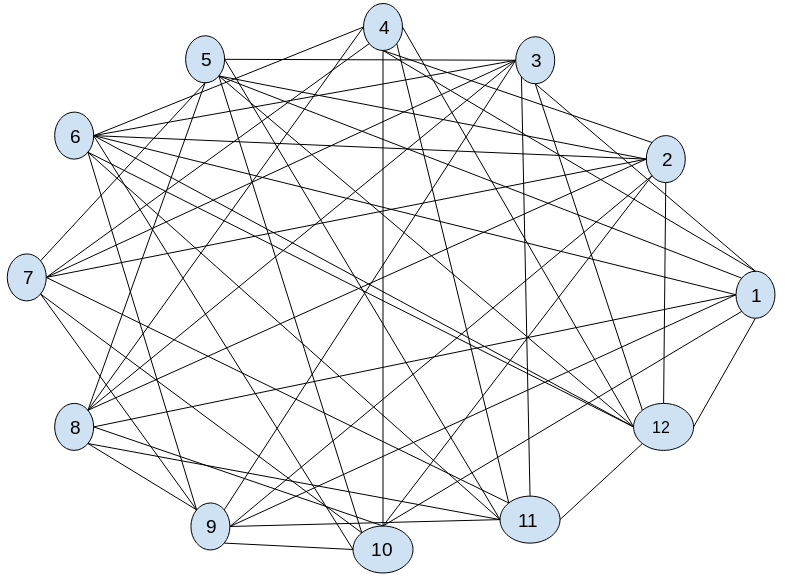
\includegraphics[scale=0.7]{frucht-compl.png}
  \end{figure}
\end{center}

Nous allons faire tourner cet algorithme pour trouver une clique d'au moins $k=5$. \\
Pour i=1 et i=2 nous trouvons des cliques de taille 4 donc nous passons à i=3.
Initialisation : $Q_3=\{i\}=\{3\}$. \\
Nous exécutons la fonction \textit{Expand\_Clique}
\begin{center}
  \begin{tabular}{|c|c|c|}
    \hline
    sommet $v$ joignable à $Q_3$ & sommets joignables à $Q_3\cup\{v\}$ & taille \\ \hline
    \hline
    1 	& 5, 6, 8, 9, 12  	& 5 \\ \hline
    5   & 1, 7, 8, 11, 12   & 5 \\ \hline
    6 	& 1, 9, 11, 12  	  & 4 \\ \hline
    7 	& 5, 9, 11, 12  	  & 4 \\ \hline
    8 	& 1, 5, 9, 11 	    & 4 \\ \hline
    9 	& 1, 6, 7, 8, 11 	  & 5 \\ \hline
    11 	& 5, 6, 7, 8, 9, 12 & 6 \\ \hline
    12 	& 1, 5, 6, 7, 11  	& 5 \\ \hline
  \end{tabular}
\end{center}
Nous trouvons que le maximum est :
\begin{displaymath}
  |Q_3 \cup \{v\}|_{max}=6 \quad pour \quad v=11
\end{displaymath}
Nous ajoutons le sommet $6$ à $Q$. Nous retrouvons la nouvelle clique \\
$Q_3=\{3, 11\}$ de taille 2.
\begin{center}
  \begin{tabular}{|c|c|c|}
    \hline
    sommet $v$ joignable à $Q_3$ & sommets joignables à $Q_3\cup\{v\}$ & taille \\ \hline
    \hline
    5 	& 7, 8, 12 	& 3 \\ \hline
    6 	& 9, 12 	  & 2 \\ \hline
    7 	& 5, 9, 12 	& 3 \\ \hline
    8 	& 5, 9 	    & 2 \\ \hline
    9 	& 6, 7, 8 	& 3 \\ \hline
    12 	& 5, 6, 7 	& 3 \\ \hline
  \end{tabular}
\end{center}
Nous trouvons que le maximum est :
\begin{displaymath}
  |Q_3 \cup \{v\}|_{max}=3 \quad pour \quad v=5
\end{displaymath}
Nous ajoutons le sommet $5$ à $Q$. Nous retrouvons la nouvelle clique \\
$Q_3=\{3, 5, 11\}$ de taille 3.
\begin{center}
  \begin{tabular}{|c|c|c|}
    \hline
    sommet $v$ joignable à $Q_3$ & sommets joignables à $Q_3\cup\{v\}$ & taille \\ \hline
    \hline
    7 	& 12 	            & 1 \\ \hline
    8 	& $ \varnothing$ 	& 0 \\ \hline
    12 	& 7 	            & 1 \\ \hline
  \end{tabular}
\end{center}
Nous trouvons que le maximum est :
\begin{displaymath}
  |Q_3 \cup \{v\}|_{max}=1 \quad pour \quad v=7
\end{displaymath}
Nous ajoutons le sommet $12$ à $Q$. Nous retrouvons la nouvelle clique \\
$Q_3=\{3, 5, 7, 11\}$ de taille 4.
\begin{center}
  \begin{tabular}{|c|c|c|}
    \hline
    sommet $v$ joignable à $Q_3$ & sommets joignables à $Q_3\cup\{v\}$ & taille \\ \hline
    \hline
    12    & $\varnothing$ & 0 \\ \hline
  \end{tabular}
\end{center}
Nous trouvons que le maximum est :
\begin{displaymath}
  |Q_3 \cup \{v\}|_{max}=0 \quad pour \quad v=12
\end{displaymath}
Nous ajoutons le sommet $12$ à $Q$. Nous retrouvons la nouvelle clique \\
$Q_3=\{3, 5, 7, 11, 12\}$ de taille 5.\\
Puisque la clique est de taille 5, nous nous arrêtons là.
\textbf{FIX THE VERTICES NAMING}
\section{Implémentation}
Nous implémentons en C++ l'algorithme trouvé précédemment pour trouver la clique
maximum d'un graphe.

\section{Performance}

\end{document}
